\documentclass{beamer}

\usepackage{beamer_tom}

\usepackage{amsfonts}


\usepackage{array}
\usepackage{xcolor,colortbl}
\newcolumntype{a}{ >{\columncolor{blue}} c }

\usepackage{tikz}
\usepgflibrary{shapes.arrows}

\graphicspath{{./images/}}

\institute{INRIA Saclay}
\author{Thomas Moreau}
\title{
    SHINE: Sharing the Inverse Estimate for bi-level optimization.
}

\setbeamertemplate{title page}[frame]
\def\extraLogo{}
\collaborators{Z. Ramzi, S. Bai, F. Mannel, J.-L. Starck \& P. Ciuciu}

\newcommand{\citeline}[1]{\textcolor{gray}{\small[{\color{linkcolor} #1}]}}
\newcommand{\blue}[1]{\textcolor{blue}{#1}}
\newcommand{\red}[1]{\textcolor{red}{#1}}


\def\biblio{
	\nobibliography{library}
	\def\biblio{}
}

\begin{document}

    \begin{frame}
        \titlepage
    	\biblio{}
    \end{frame}


    \frame{
        \frametitle{Learning a linear ML model}


        \textbf{Setup:}\\[1em]
        \begin{itemize}
            \item Binary classification task $(X_i, y_i)_{i=1}^N \in \mathbb R^p \times \{-1, 1\}$
            \item Linear model: predict $y$ from $X$ with $\text{sign}(\langle \theta, X\rangle)$.
        \end{itemize}

        {\centering
        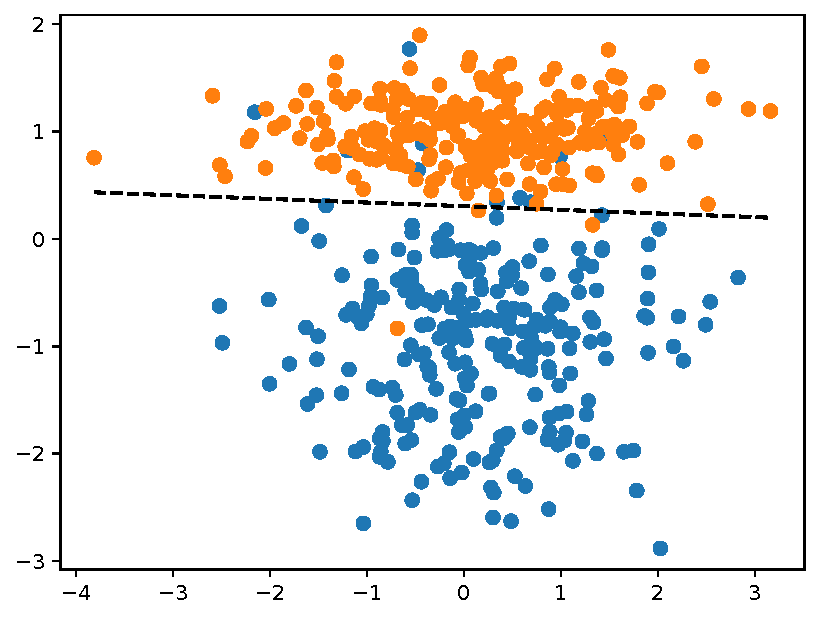
\includegraphics[width=.6\textwidth]{images/logreg_noreg}\\
        }

    }

    \frame{
        \frametitle{$\ell_2$-regularized logistic regression}
        \textbf{{Regularized} Logistic loss:}

        \[
            G(\lambda, \theta) = \frac1N \sum_{i=1}^N \log( 1 + e^{-y_i \langle \theta, X_i\rangle}) + \lambda\|\theta\|_2^2
        \]


        \textbf{Training the model:}\\[1em]
        \[
            \theta^*(\lambda) = \argmin_\theta G(\lambda, \theta)
        \]

        \pause
        \strongpoint{\bf Choose $\lambda$ using validation data.}

    }

    \frame{
        \frametitle{Evaluating the generalization}

        We want to find $\lambda$ that ensure the best \emph{generalization} of $\theta^*(\lambda)$.\\[2em]

        \textbf{Validation loss:} use held out data $(X^{\it val}_i, y^{\it val}_i)_{i=1}^M$
        \[
            F(\theta) = \frac1M \sum_{i=1}^M \log( 1 + e^{-y^{\it val}_i \langle \theta, X_i^{\it val}\rangle})
        \]

        Independent estimate of the risk of the model.\\[1em]

        \pause
        \strongpoint{Find $\lambda$ that gives a model $\theta^*(\lambda)$ with a good validation loss.}

        \vskip2em
        \textbf{Mathematical rewritting:}
        $\begin{cases}
            \quad\min_{\lambda}
            F(\theta^*(\lambda))\\
            s.t.\quad \theta^*(\lambda) = \argmin_\theta G(\lambda, \theta)
        \end{cases}$
    }

    \frame{
        \frametitle{Bi-level optimization}

        {\bf Bi-level problem:} Optimization problem with two levels\\[1em]
        \begin{align*}
            \min_\lambda ~& {\color{darkblue} h(\lambda)} = {\color{darkred}F(\lambda, \theta^*(\lambda))} \\[.5em]
                & s.t.\quad \theta^*(\lambda) = \argmin_\theta {\color{lightgreen}G(\lambda, \theta)}
        \end{align*}
        \begin{tikzpicture}[overlay]
            \draw[<-, thick, shorten >=8, darkblue] (4.1, 1.7) -- +(-1.5, -1.3) node[darkblue] {\emph{Value function}};
            \draw[<-, thick, shorten >=35,darkred] (7.3, 1.9) -- +(3, -.2) node {\emph{\color{darkred}Outer function}};
            \draw[<-, thick, shorten >=8, lightgreen] (8, .5) -- +(0, -.8) node {\emph{\color{lightgreen} Inner function/Problem}};
        \end{tikzpicture}

        \vskip3em
        {\bf Goal:}  Optimize the value function $h$ whose value depends on the result of another optimization problem.
    }
    \frame[t]{
        \frametitle{Bi-level optimization problems: Model selection}

        \vskip1em
        {\bf Selecting the best model:}\\[.5em]
        \begin{itemize}\itemsep.7em
            \item $G$ is the training loss and $\theta$ are the parameters of the model.
            \item Select the hyper-parameter $\lambda$ to get the best validation loss $F$.
        \end{itemize}
        \vskip1em
        \alt<2->{
            \alt<3>{
                {\bf Neural Architecture Search:} $\lambda$ parametrizes the architecture. \\

                {\centering
                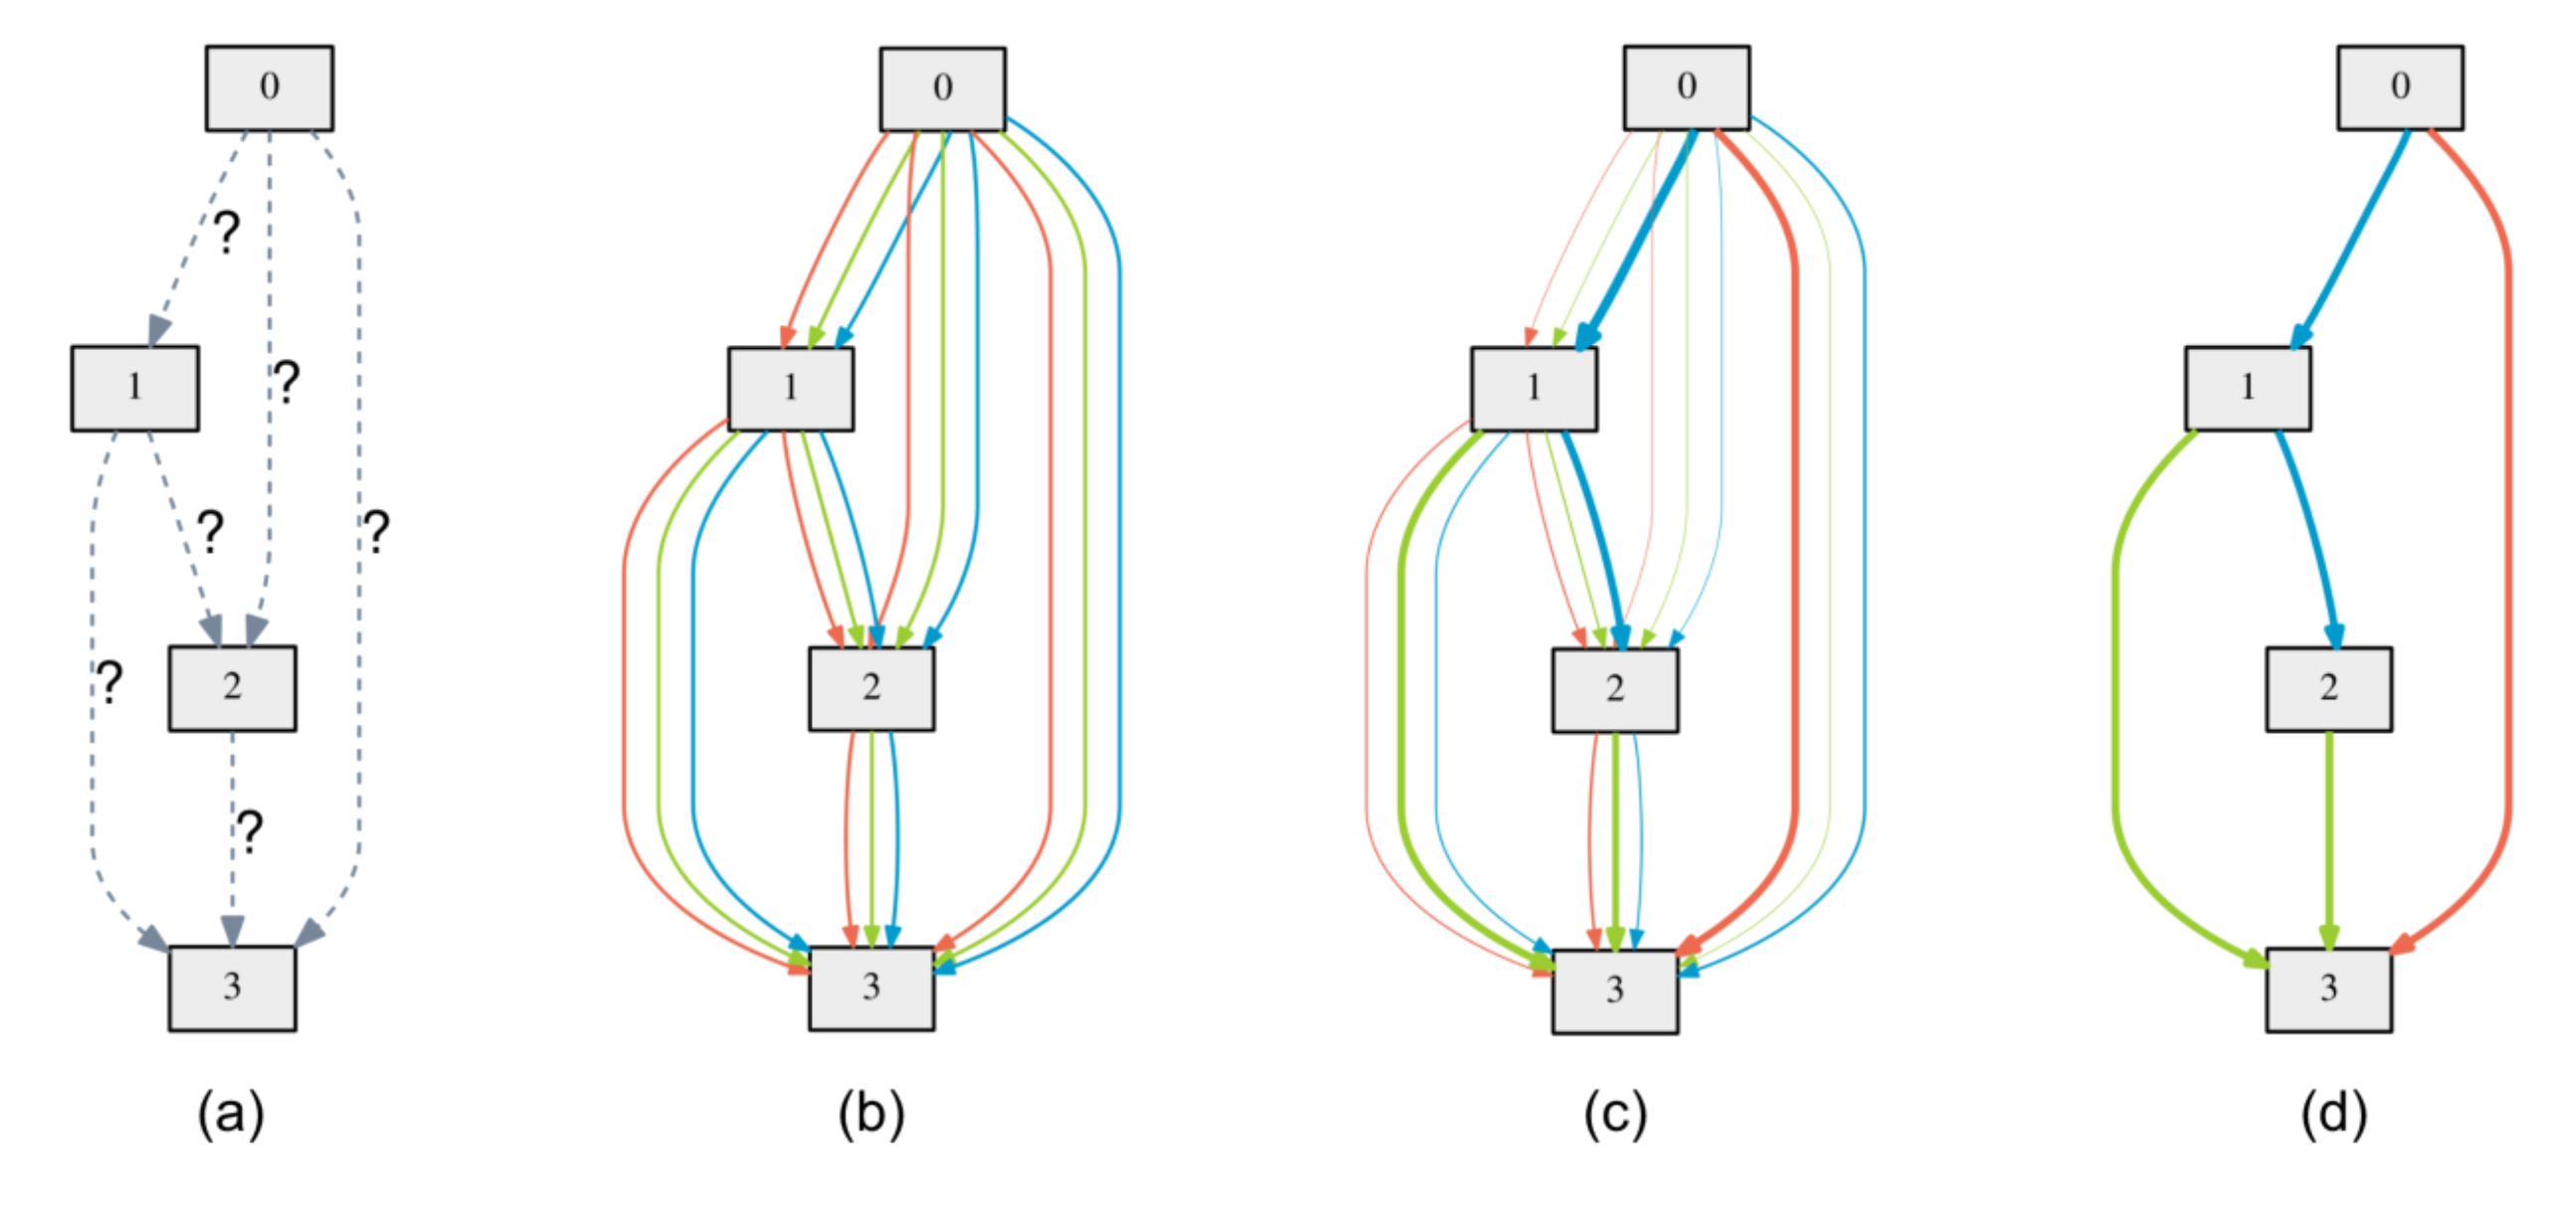
\includegraphics[width=.8\textwidth]{darts.png}\\
                }

            }{
                {\bf Data augmentation:} $\lambda$ parametrizes the transformations distribution. \\

                {\centering
                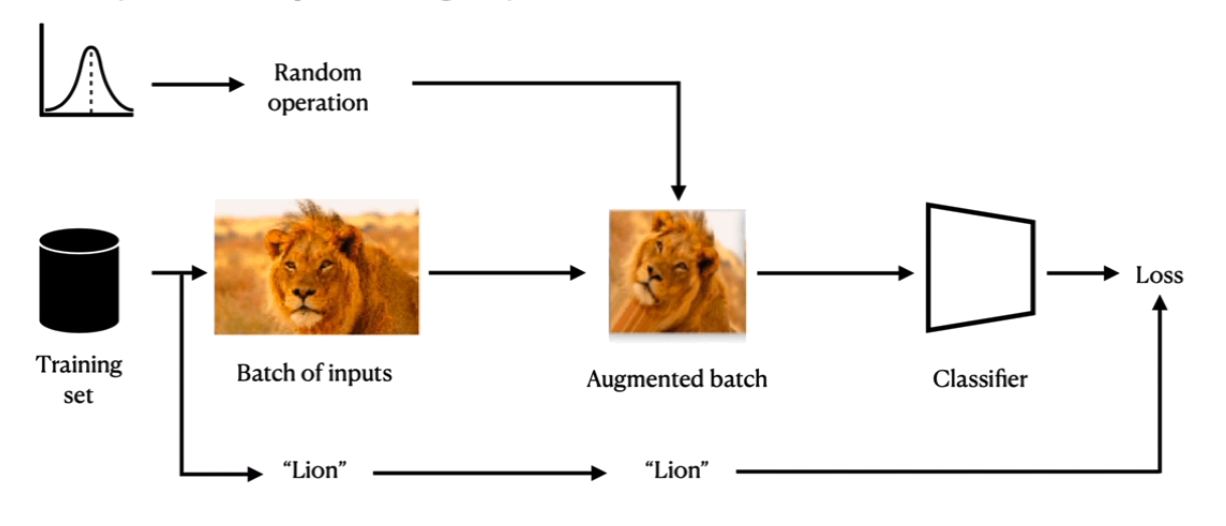
\includegraphics[]{data_aug.png}\\
                }
            }
        }{
            {\bf Hyperparameter optimization:} $\lambda$ is a regularization parameter:\\[1em]

            {\centering
            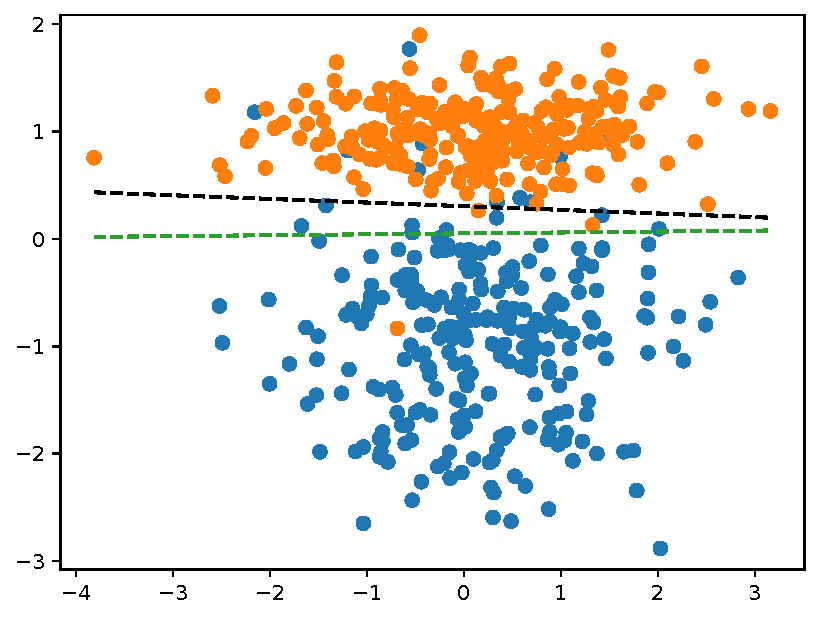
\includegraphics[width=.4\textwidth]{images/logreg_reg}\\
            }
        }

    }


    \frame{
        \frametitle{Solving bi-level optimization}

        \alt<2>{
            \vskip2em
            \underline{\bf First order methods:} Gradient descent on $h$
            \begin{columns}
                \column{.5\textwidth}
                \vskip1em
                Iterate in the steepest direction:
                $$
                    \lambda^{t+1} = \lambda^t - \rho^t \nabla h(\lambda)
                $$
                \myitem{} Gradient $\nabla h(\lambda) = \frac{d\; F(\lambda, \theta^*(\lambda))}{d\;\lambda}$\\[.5em]
                \myitem{} Step size $\rho^t$.
                \column{.5\textwidth}
                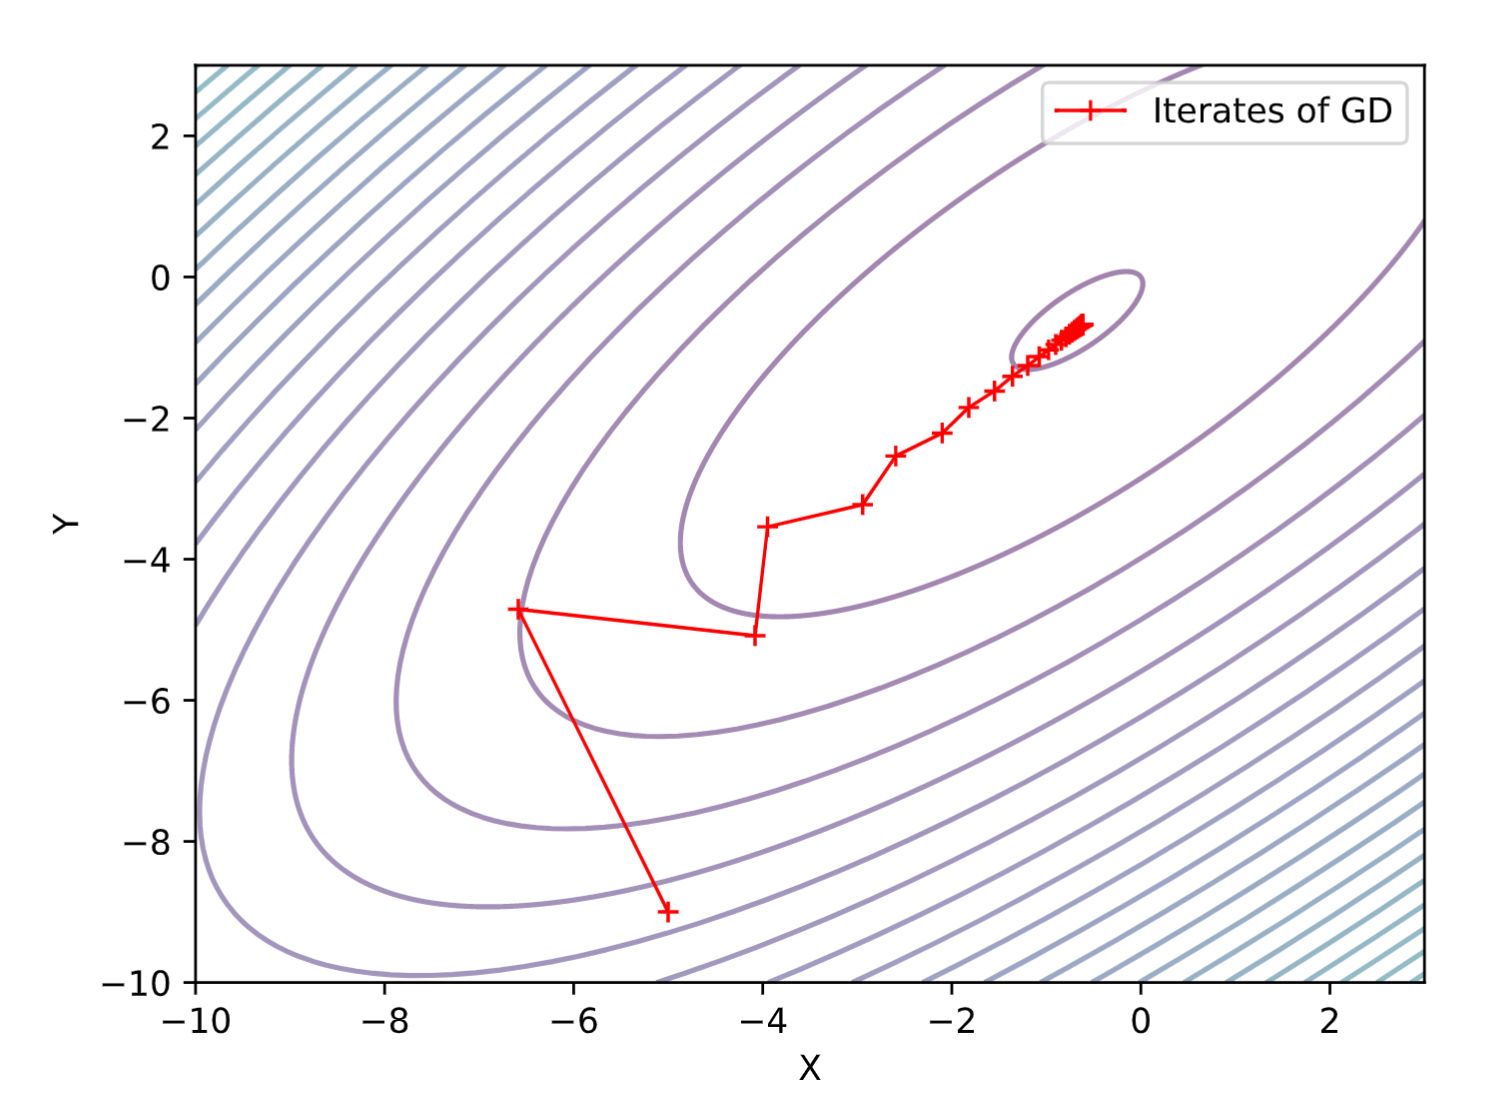
\includegraphics[width=\textwidth]{gd_Steps.png}
            \end{columns}
        }{
            \underline{\bf Black box methods:} Take $\{\lambda_k\}_k$ and compute $\min_k h(\lambda_k)$ \\[1em]
            {
                \centering
                \myitem{} Grid-Search
                \hskip4ex
                \myitem{} Random-Search
                \hskip4ex
                \myitem{} Bayesian-Optimization\\[1em]
            }
            \strongpoint{Do not scale well with the dimension}

        }

        % \pause
        % \begin{itemize}
        %     \item Can we compute the gradient of $h$?
        %     \item Do we need to compute $\theta^*(\lambda)$?\\
        %     \item How to efficiently approximate $\nabla h(\lambda)$?
        % \end{itemize}
    }

    % \frame{
    %     \frametitle{Some challenges?}


    %     \begin{itemize}\itemsep1em
    %         \item Computing the gradient of $h$?\\
    %         \rightcite{Implicit function theorem}
    %         \item Do we need to compute $z^*$?\\
    %         What is the best gradient estimate with $z_t$?\\
    %         \rightcite{Pedregosa 2016, Ablin et al. 2020, Malezieux et al. 2022}
    %         \item How to efficiently compute the implicit gradient?\\
    %         \rightcite{Lorraine et al. 2017, Ramzi et al. 2022}
    %         \item How to use stochastic methods?
    %         \rightcite{Grazzie et al. 2021, Chen et al. 2021}
    %     \end{itemize}
    % }


    % \section{Implicit Gradient}
    % \parttitleframe[Computing the gradient of the value function $h$]{Pedregosa2016,Lorraine2020,Ramzi2022}

    \frame{
        \frametitle{Computing the gradient of $h$}

        \underline{\bf{Value function definition:}}
        \[
            h(\lambda) = F(\lambda, \theta^*(\lambda))
        \]

        \underline{\bf{Chain rule:}}
        \[
            \nabla_\lambda h(\lambda) = \nabla_1 F (\lambda, \theta^*(\lambda))
            + (d \theta^*(\lambda))^T\nabla_2 F(\lambda, \theta^*(\lambda))
        \]
    }
    \frame{
        \frametitle{Jacobian of $\theta^*$ - implicit differentiation}

        \underline{\bf{Optimality condition for $\theta^*$}}
        \[
            \nabla_2 G(\lambda, \theta^*(\lambda)) = 0
        \]

        \pause
        Derivating this equation relative to $\lambda$ gives:
        \[
            \nabla^2_{22}G(\lambda, \theta^*(\lambda)) d \theta^*(\lambda) + \nabla^2_{21}G( \lambda, \theta^*(\lambda)) = 0,
        \]
        \pause

        \underline{\bf{Implicit function theorem}}
        \[
            d \theta^*(\lambda) = - \big[\nabla_{22}^2 G(\lambda, \theta^*(\lambda))\big]^{-1}\nabla_{21}^2 G(\lambda, \theta^*(\lambda)),
        \]
    }
    \frame{
        \frametitle{Computing the gradient of $h$}

        \underline{\bf{Value function gradient:}}\\[1em]
        \[
            \nabla h(\lambda) = \nabla_1 F(\lambda, {\alt<2>{\color{blue!70}}{}\theta^*})
        -  \nabla_{21}^2 G(\lambda, {\alt<2>{\color{blue!70}}{}\theta^*})
        {\alt<3>{\color{blue!70}}{}
        \big[\nabla_{22}^2G(\lambda, {\alt<2>{\color{blue!70}}{}\theta^*})\big]^{-1}\nabla_2 F(\lambda, {\alt<2>{\color{blue!70}}{}\theta^*})}
        \]

        \vskip3em
        \begin{itemize}\itemsep1em
            \item<2-> Need to compute the solution of the inner
            \item<3-> Need to solve a $p\times p$ linear system
            \[ v^*(\lambda) = \big[\nabla_{22}^2G(\lambda, \theta^*)\big]^{-1}\nabla_2 F(\lambda, \theta^*)\]
        \end{itemize}
    }

    \section{Approximate bi-level optimization}
    \parttitleframe[]{Pedregosa2016}

    \frame{
        \frametitle{Hyperparameter optimization with Approximate Gradient HOAG \rightcite{Pedregosa 2016}}

        {\centering \emph{Do we need to compute $\theta^*$ and $v^*$ precisely?}\\[1em]}

        {\bf Idea: } Approximate $\theta^*(\lambda^t)$ and $v^*(\lambda^t) = \big[\nabla_{22}^2G(\lambda^t, \theta^*)\big]^{-1}\nabla_2 F(\lambda^t, \theta^*)$\\[1em]


        \visible<2->{
        \begin{itemize}\itemsep1em
            \item Compute $\theta^t$ such that $\|\theta^t - \theta^*(\lambda^t)\|_2 \le \epsilon_t$, \\
                \keypoint{iterative solver \emph{e.g.} L-BFGS}
            \item Compute $v^t$ such that $\|\frac{\partial^2G}{\partial \theta^2}(\lambda^t, \theta^t)v^t + \frac{\partial F}{\partial \theta}(\lambda^t, \theta^t)\|_2 \le \epsilon_t$,\\
            \keypoint{L-BFGS or CG}
            \item Compute the approximate gradient $g_t = \frac{\partial F}{\partial \lambda} (\lambda^t, \theta^t)
            + \frac{\partial^2 G}{\partial \theta\partial\lambda}(\lambda^t, \theta^t) v^t$
            \item Update the outer variable $\lambda^{t+1} = \lambda^t - \rho^t g^t$
        \end{itemize}
        \vskip1em
        }
    }

    \frame{
        \frametitle{HOAG \rightcite{Pedregosa 2016}}
        {\bf Theorem: } If $\sum_t \epsilon_t < \infty$ and the step-sizes are chosen appropriatly, then the algorithm converges to a stationary point \emph{i.e.}
        $$
            \|\nabla h(\lambda^t)\|_2 \to 0 \enspace.
        $$
    }


    \frame{
        \frametitle{Further linear system approximation $v^*$}

        Linear system solution $v^*(\lambda^t)$ is a by product.

        \strongpoint{Avoid computing it as much as possible.}

        \vskip2em
        \underline{\bf Proposed Methods:}\\[1em]
        \begin{columns}[T]
            \column{.4\linewidth}
            \myitem{} L-BFGS\\[1em]
            \myitem{} Jacobian-Free method
            \[
                \phantom{\sum_k}\nabla_{22}^2 G(\lambda^t, \theta^t) \approx Id
            \]

            \myitem{} Algorithm unrolling
            \column{.6\linewidth}
            \myitem{} Conjugate Gradient\\[1em]
            \myitem Neumann iterations
            \[
                \nabla_{22}^2 G(\lambda^t, \theta^t)^{-1}\approx \sum_k (Id - \nabla_{22}^2 G(\lambda^t, \theta^t))^k
            \]
            \myitem{} Use Quasi-newton hessian approximation
        \end{columns}
        \vspace{0pt plus 1 filll}
        \rightcite{Pedregosa 2016, Lorraine et al. 2020, Luketina et al. 2016, Ramzi et al. 2022}


    }



    \section{SHINE - Sharing the INverse Estimate}
    \parttitleframe{Ramzi2022}

    \frame{
        \frametitle{SHINE: SHaring the INverse Estimate
                    \rightcite{Ramzi et al. 2022}}

        \underline{\bf Quasi Newton 101:}\\[1em]
        {\centering Solving $\theta^* = \argmin_\theta G(\theta)$\\[2em]}
        \begin{columns}[T]
            \column{.5\linewidth}
            {\centering \bf Newton Method\\}
            \[
                \theta^{t+1} = \theta^t - \big[\nabla^2G(\theta^t)\big]^{-1}\nabla G(\theta^t)
            \]

            \column{.5\linewidth}
            {\centering \bf Quasi-Newton Method\\[.7em]}
            \[
                \theta^{t+1} = \theta^t - B_t^{-1}\nabla G(\theta^t)
            \]
            $B_t$: low-rank approx. of $\nabla^2G(\theta^t)$.\\
            \keypoint{Inverse with Sherman-Morrison}
        \end{columns}

        \pause
        \strongpoint{The Hessian for $v^*$ is the same as the one from the inner problem.}
    }

    \frame{
        \frametitle{SHINE - Hyper-parameter optimization \rightcite{Ramzi et al. 2022}}

        {\bf Idea:} \parbox[t]{.8\textwidth}{reuse the approximation of the Hessian $B_t$ computed\\
            by L-BFGS for the inner problem.}
        \[
            \begin{cases}
                \tilde{v}_t = B_t^{-1}\nabla_2 F(\lambda, \theta^t)\\
                \tilde\nabla h(\lambda) = \nabla_1 F(\lambda, \theta^t) + \nabla_{12}^2G(\lambda, \theta^t)\tilde{v}_t
            \end{cases}
        \]

        \underline{\bf Properties of $B$:}\\[1em]
        \begin{itemize}
            \item<2-> It is computed when solving $\theta^* = \argmin_\theta G(\theta)$ using a quasi-Newton method.
            \item<3-> It is easily invertible using the Sherman-Morrison formula, because low-rank.
        \end{itemize}

    }

    \begin{frame}{SHINE direction convergence}
        \begin{theorem}[Convergence of SHINE to the Hypergradient using ULI]
            Under the Uniform Linear Independence~(ULI) assumption and some additional smoothness and convexity assumptions, for a given parameter $\lambda$, $(\theta^t)$ converges q-superlinearly to $\theta^\star$ and
            \begin{equation*}
                \lim_{t \to \infty} \nabla_1 F(\lambda, \theta^t) + \nabla_{12}^2G(\lambda, \theta^t)\tilde{v}_t = \nabla h(\lambda).
            \end{equation*}
            \end{theorem}
    \end{frame}

    % \frame{
    %     \frametitle{Outer Problem Awarness \rightcite{Ramzi et al. 2022}}

    %     To relax these conditions, we propose the OPA algorithm
    % }

    \frame{
        \frametitle{SHINE - Hyper-parameter optimization \rightcite{Ramzi et al. 2022}}

        Logistic Regression with $\ell_2$-regularisation on 2 datasets:\\[1em]

        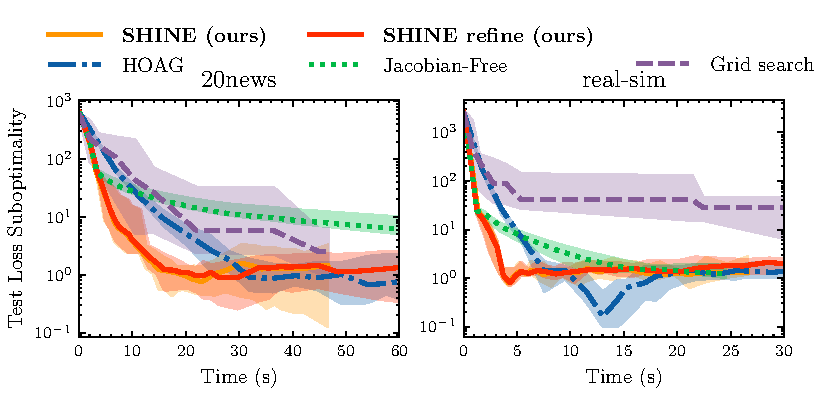
\includegraphics[width=\textwidth]{bilevel_test.pdf}\\
    }


\section{Application to Deep Equilibrium Networks (DEQs)}
\parttitleframe{}


\begin{frame}{Infinite depth neural networks}
    A recurrent expression of classical, explicit networks:
    % \only<1>{
    %     \begin{center}
    %         \begin{tikzpicture}[
    %             font=\Large, node distance=2.5em,>=stealth,
    %             function/.style={circle,draw},
    %         ]
    %             % nodes
    %             \begin{scope}[execute at begin node=$, execute at end node=$]
    %                 \node (input_node) {x};
    %                 \node (first_int_function) [right=of input_node, function] {f_{\lambda_1}};
    %                 \node (dots) [right=of first_int_function] {\ldots};
    %                 \node (last_int_function) [right=of dots, function] {f_{\lambda_N}};
    %                 \node (output_node) [right=of last_int_function] {\hat{y}};
    %             \end{scope}

    %             % arrows
    %             \draw[->] (input_node) -- (first_int_function);
    %             \draw[->] (first_int_function) -- (dots) node (first_activation) [above,midway] {$\theta_1$};
    %             \draw[->] (dots) -- (last_int_function) node (last_activation) [above,midway] {$\theta_{N-1}$};
    %             \draw[->] (last_int_function) -- (output_node);

    %         \end{tikzpicture}
    %     \end{center}

    % }
    \only<1->{
        \begin{equation*}
            \theta_{n} = f_{\lambda_{n}}(\theta_{n-1}), \quad \forall n < N
        \end{equation*}
    }

    \onslide<2->{
        What if $N \to \infty$?

        If we suppose $\lambda_{n} = \lambda, \forall n$:
        \begin{equation*}
            \theta^\star = f_{\lambda}(\theta^\star)
        \end{equation*}
    }

    \end{frame}


\begin{frame}{Deep Equilibrium networks}
    % give equation and how to compute the gradient with IFT
    % \citet{Bai2019DeepModels} introduced \textbf{Deep Equilibrium networks~(DEQs)}, a type of implicit model.
    \textbf{Deep Equilibrium networks~(DEQs)}~\citep{Bai2019} are a type of implicit model.
    % The output of DEQs is defined implicitly as the solution to a fixed-point equation.
    The output is the solution to a fixed-point equation.

    % XXX: have directly g formulation
    \begin{equation*}
        h_{\lambda}(x) = \theta^\star, \text{ where }
        % \alt<3>{g_\lambda(\theta^\star, x) = \theta^\star - f_\lambda(\theta^\star, x) = 0}{
        \theta^\star = f_\lambda(\theta^\star, x)
    \end{equation*}

    \visible<2->{
        \vskip1em
        This approximates an infinite depth network:
        \begin{equation*}
            \theta_{n} = f_{\lambda}(\theta_{n-1}), \quad \forall n \to \infty
        \end{equation*}

        In practice, we work with root finding algorithms using $g_\lambda = id - f_\lambda$.
    }


    % In practice, we solve this equation with a \textbf{quasi-Newton method}.
    % In practice, solved with a \textbf{quasi-Newton method}.
\end{frame}



    \frame{
        \frametitle{Bi-level optimization problems: Implicit Deep Learning}

        {\bf Deep Equilibrium Network:}
        \[
            \begin{cases}
            \min_\lambda h(\lambda) = \frac1N\sum_{i=1}^N \mathcal L(y_i, \theta^*(X_i, \lambda))\\
            s.t.\quad \theta^*(X_i, \lambda) = g_\lambda(\theta^*(X_i, \lambda))
            \end{cases}
        \]
        Output of the network is the root of $G(\theta, \lambda) = \theta - g_\lambda(\theta) =0$.\\[2em]

        In pratice, use quasi-Newton algorithm such as the Broyden method for both finding $\theta^*$ and its derivative $v^*$.
    }

    \frame{
        \frametitle{Deep Equilibrium Network}
        \centering
        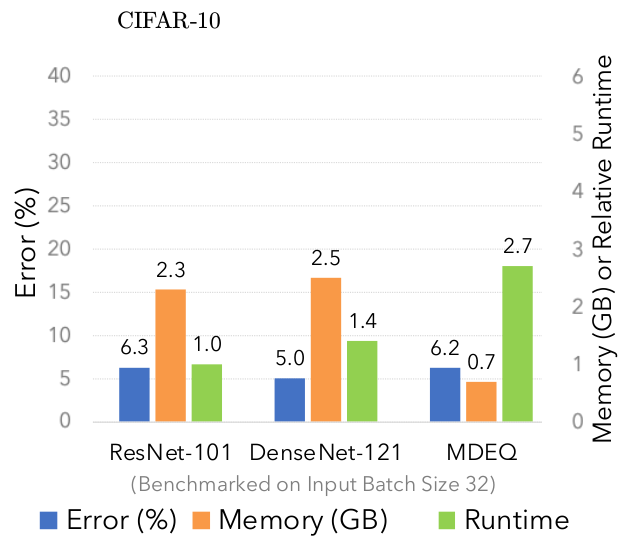
\includegraphics[width=.6\textwidth]{deq_memory.png}\\[2em]
        \myitem{} {\bf Efficient memory}\hskip3em
        \myitem{} {\bf Slow runtime}\\
    }


    \frame{
        \frametitle{SHINE - DEQ \rightcite{Ramzi et al. 2022}}

        Multiscale DEQ on CIFAR10:\\[1em]

        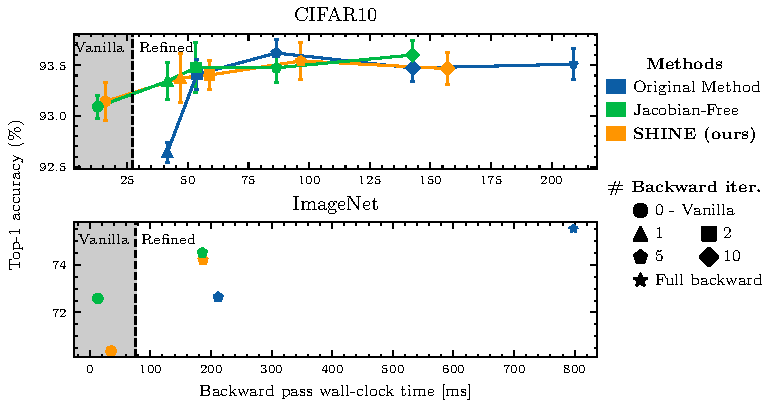
\includegraphics[width=\textwidth]{mdeq.pdf}\\
    }

    \frame{
        \frametitle{OPA - Outer Problem Awarness}

        $B^{-1}$ is not a uniformly good approximation.\\[1em]
        {\bf OPA:} add additional secant conditions for $B$ update.
            \centering
        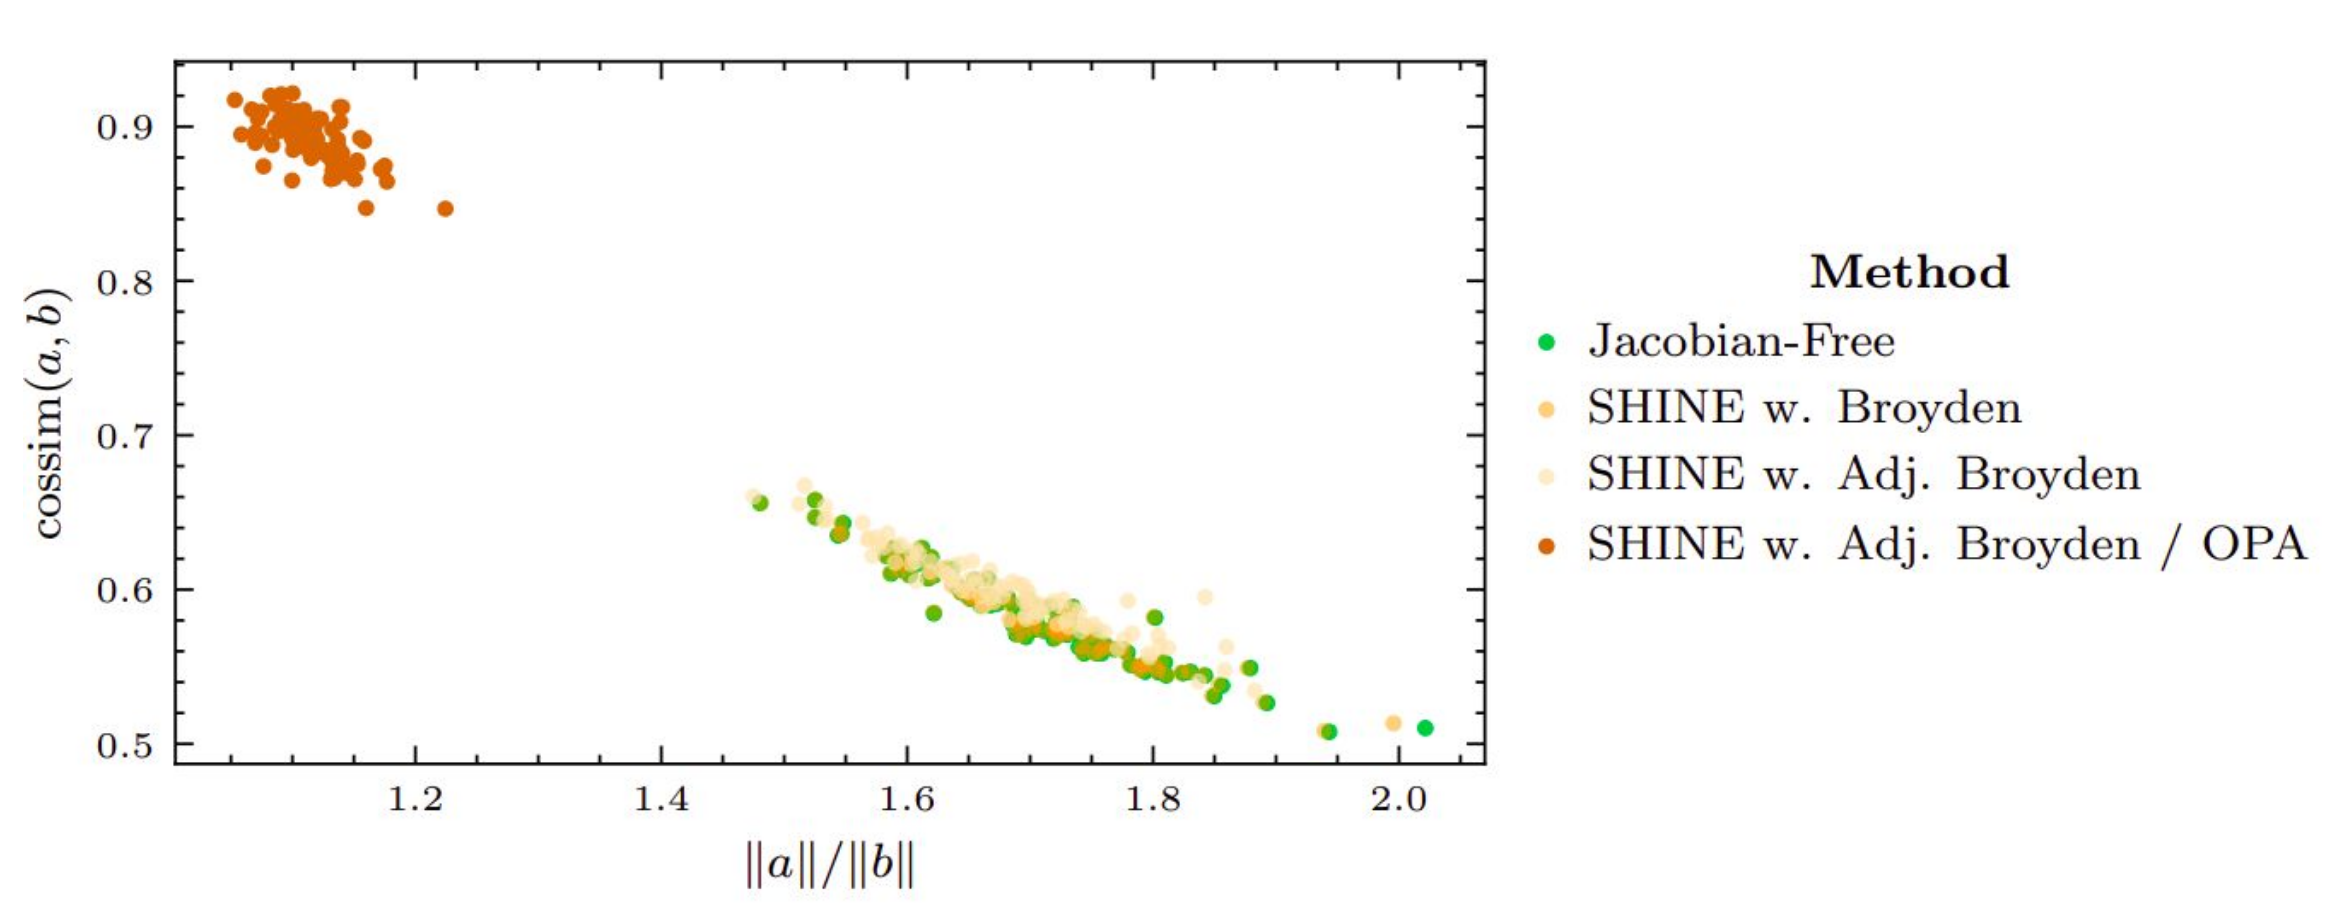
\includegraphics[width=.9\textwidth]{opa}\\[1em]

        \strongpoint{Better gradient approximation (theoretical and empirical)}
        \vskip1em
        However, this does not improve results for test error.
    }


\frame{
    \frametitle{Conclusion}

    \vspace{0pt plus 1 filll}
    \begin{itemize}\itemsep1em
        \item Bi-level optimization is intrinsic in many ML problems.
        \item We propose to re-use by-product from $\theta^*$ computation to make it easy to get $v^*$.
        \item Good results for HO but still open questions for DEQs.
    \end{itemize}



    {\vskip2em\centering
    \includegraphics[height=5em]{People/zramzi}\hskip1em
    \includegraphics[height=5em]{People/sbai}\hskip1em
    \includegraphics[height=5em]{People/fmannel}\hskip1em
    \includegraphics[height=5em]{People/jlstarck}\hskip1em
    \includegraphics[height=5em]{People/pciuciu}\\
    Z. Ramzi\hskip3em S. Bai\hskip2em F. Mannel\hskip2em J.L. Starck\hskip2em P. Ciuciu\\}

    \vspace{0pt plus 1 filll}
    Slides will be on my web page:\\[.5em]
    \hskip5em\includegraphics[height=.8em]{website} \url{tommoral.github.io}
    \hskip4em 
\includegraphics[height=.8em]{twitter} \href{https://twitter.com/tomamoral}{@tomamoral}\\

    }

\end{document}
